\documentclass{standalone}

\usepackage{microtype}
\usepackage[utf8]{inputenc}
\usepackage[mono=false]{libertine}

\usepackage{pgfplots}
\usepgfplotslibrary{external}

\usepackage{tikz}
\usetikzlibrary{shapes.geometric, arrows, calc}

\newcommand{\cdicov}{$19\,670$}

\newcommand{\cdiagepcg}{$23.7$}
\newcommand{\cdisexpcg}{$-41.3$}
\newcommand{\cdibopcg}{$73.5$}
\newcommand{\cdivrspcg}{$-8.3$}

\newcommand{\cdiagescg}{$23.2$}
\newcommand{\cdisexscg}{$-45.2$}
\newcommand{\cdiboscg}{$54.2$}
\newcommand{\cdivrsscg}{$-9.1$}

\newcommand{\bapqcov}{$0.05$}
\newcommand{\gendercov}{$-0.2$}
\newcommand{\educcov}{$0.32$}
\newcommand{\tswccov}{$26.4$}

\newcommand{\bapqpcg}{$-22.5$}
\newcommand{\bapqscg}{$-3.7$}

% format: pcg/scg outcome~cov

\newcommand{\pcgedgender}{$-1.02$}
\newcommand{\pcgedbapq}{$-1.23$}
\newcommand{\pcgtswcgender}{$-5.25$}
\newcommand{\pcgtswced}{$-0.67$}

\newcommand{\scgedgender}{$-1.14$}
\newcommand{\scgedbapq}{$-3.89$}
\newcommand{\scgtswcgender}{$-1.3$}
\newcommand{\scgtswced}{$-0.07$}

\newcommand{\vrrsbage}{$-0.8$}
\newcommand{\vrrsbsex}{$2.0$}

\newcommand{\ns}{\textsuperscript{n.s.}}

%\tikzexternalize[prefix={tikz_external/}, only named]
%\tikzsetnextfilename{vrs}

\definecolor{cdired}{HTML}{FF8080}
\definecolor{pcgcolor}{HTML}{E070DA}
\definecolor{scgcolor}{HTML}{70DAE0}
\definecolor{childcolor}{HTML}{DAE070}

\tikzstyle{outcome} = [rectangle, draw=black]
\tikzstyle{child} = [rectangle, rounded corners, fill=childcolor, draw=black]
\tikzstyle{p1} = [rectangle, rounded corners, fill=pcgcolor, draw=black]
\tikzstyle{p2} = [rectangle, rounded corners, fill=scgcolor, draw=black]

\tikzstyle{arrow} = [thick,->]
\tikzstyle{dblarr} = [thick,<->]

\begin{document}

    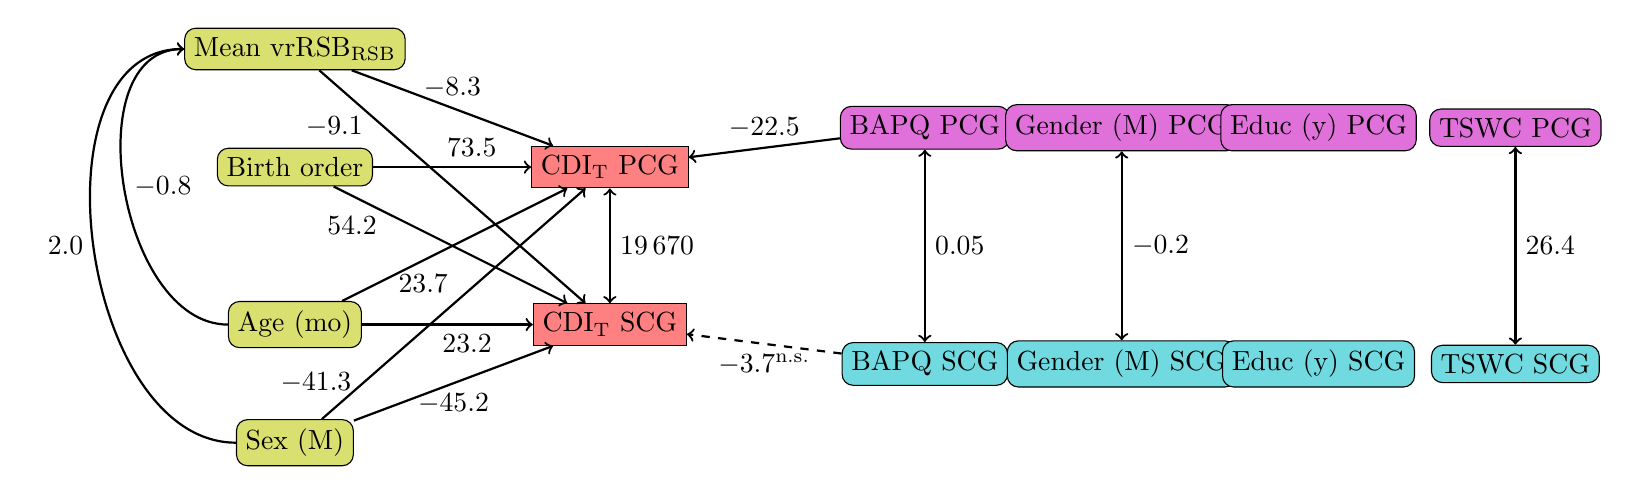
\begin{tikzpicture}

        \node (cdi1) [outcome, fill=cdired] {CDI\textsubscript{T} PCG};
        \node (cdi2)
            [outcome, fill=cdired, below of=cdi1, node distance=2cm]
            {CDI\textsubscript{T} SCG};

        \node (center) at ($(cdi1)!0.5!(cdi2)$) {} ;

        % Place this stack of nodes to the left of the center of the things
        \node (age)
            [child, left of=cdi2, node distance=4cm]
            {Age (mo)} ;
        \node (bo)  [child, left of=cdi1, node distance=4cm] {Birth order} ;
        \node (sex) [child, below of=age, node distance=1.5cm] {Sex (M)} ;
        \node (vrs) [child, above of=bo, node distance=1.5cm]
            {Mean vrRSB\textsubscript{RSB}} ;

        % arrows
        \draw [dblarr] (cdi1) -- node[anchor=west] {\cdicov} (cdi2) ;

        \draw [arrow] (age) --
            node[anchor=north,yshift=-0.25cm,xshift=-0.4cm] {\cdiagepcg}
            (cdi1) ;
        \draw [arrow] (age) --
            node[anchor=north,xshift=0.25cm] {\cdiagescg}
            (cdi2) ;

        \draw [arrow] (sex) --
            node[anchor=north,yshift=-0.75cm,xshift=-1.75cm] {\cdisexpcg}
            (cdi1) ;
        \draw [arrow] (sex) --
            node[anchor=north]
             {\cdisexscg} (cdi2) ;

        \draw [arrow] (bo) --
            node[anchor=south,xshift=0.25cm] {\cdibopcg}
            (cdi1) ;
        \draw [arrow] (bo) --
            node[anchor=south,xshift=-1.25cm] {\cdiboscg}
            (cdi2) ;

        \draw [arrow] (vrs) -- node[anchor=south] {\cdivrspcg} (cdi1) ;

        \draw [arrow] (vrs) --
            node[anchor=south,yshift=0.5cm,xshift=-1.5cm] {\cdivrsscg}
            (cdi2) ;

        \draw [arrow] (age) to
            [out=180,in=180]
            node[anchor=west] {\vrrsbage}
            (vrs) ;
        \draw [arrow] (sex) to
            [out=180,in=180]
            node[anchor=east] {\vrrsbsex}
            (vrs) ;

%        % PARENTS ====
%
        \node (parentcenter) [right of=center, node distance=4cm] {} ;

        \node (p1bapq) [p1, above of=parentcenter, node distance=1.5cm]
            {BAPQ  PCG} ;
        \node (p1gender) [p1, right of=p1bapq, node distance=2.5cm]
            {Gender (M) PCG} ;
        \node (p1educ) [p1, right of=p1gender, node distance=2.5cm]
            {Educ (y) PCG} ;
        \node (p1tswc) [p1, right of=p1educ, node distance=2.5cm] {TSWC PCG} ;

        \node (p2bapq) [p2, below of=parentcenter, node distance=1.5cm]
            {BAPQ SCG} ;
        \node (p2gender) [p2, right of=p2bapq, node distance=2.5cm]
            {Gender (M) SCG} ;
        \node (p2educ) [p2, right of=p2gender, node distance=2.5cm]
            {Educ (y) SCG} ;
        \node (p2tswc) [p2, right of=p2educ, node distance=2.5cm] {TSWC SCG} ;

        \draw [dblarr] (p1bapq) --   node[anchor=west] {\bapqcov} (p2bapq) ;
        \draw [dblarr] (p1gender) -- node[anchor=west] {\gendercov} (p2gender) ;
        %        \draw [dblarr] (p1educ) --   node[anchor=west] {\educcov}
%(p2educ) ;
        \draw [dblarr] (p1tswc) --   node[anchor=west] {\tswccov} (p2tswc) ;
%
%        % PCG
%
%        %        \draw [->] (p1gender) to [bend left, out=30, in=150] (p1bapq) ;
%        \draw [->]
%        (p1gender) to
%        [bend right]
%        node[anchor=north]{\pcgedgender}
%        (p1educ) ;
%
%        \draw [->,dashed]
%        (p1bapq) to
%        [out=30,in=150]
%        node[anchor=south] {\pcgedbapq\ns}
%        (p1educ) ;
%
%        \draw [->] (p1educ) to
%        [bend right]
%        node[anchor=north] {\pcgtswced}
%        (p1tswc) ;
%
%        \draw [->] (p1gender) to
%        [out=30,in=150]
%        node[anchor=south] {\pcgtswcgender}
%        (p1tswc) ;
%
%        %        \draw [<->,dotted] (p2educ) to
%        %            [out=30,in=150]
%        %            (p2bapq) ;
%
%        % SCG
%
%        %        \draw [->] (p2gender) to [out=150, in=30] (p2bapq) ;
%        \draw [->]
%        (p2gender) to
%        [bend left, out=30,in=150]
%        node[anchor=south] {\scgedgender}
%        (p2educ) ;
%
%        \draw [->]
%        (p2bapq) to
%        [bend right]
%        node[anchor=north] {\scgedbapq}
%        (p2educ) ;
%
%        \draw [->,dashed]
%        (p2educ) to
%        [bend left]
%        node[anchor=south] {\scgtswced\ns}
%        (p2tswc) ;
%
%        \draw [->,dashed]
%        (p2gender) to
%        [bend right]
%        node[anchor=north] {\scgtswcgender\ns}
%        (p2tswc) ;
%
%        % bapq effects
        \draw [arrow] (p1bapq) -- node[anchor=south] {\bapqpcg} (cdi1) ;
%
        \draw [arrow,dashed] (p2bapq)
            -- node[anchor=north] {\bapqscg{}\ns{}}
        (cdi2) ;

    \end{tikzpicture}


\end{document}